%  after submission
%
% 
%
%
%
%
%
%
\documentclass{llncs} %

\usepackage{pslatex}
\usepackage{apacite}
\usepackage{url}
\usepackage{graphicx}
\usepackage{listings}
\usepackage{color}
\usepackage{textcomp}
\usepackage{amsmath}
\usepackage{amssymb}
\usepackage{wrapfig}
\usepackage{lipsum}

 \newcommand{\denote}[1]{\mbox{ $[\![ #1 ]\!]$}}

\definecolor{Red}{RGB}{255,0,0}
\newcommand{\red}[1]{\textcolor{Red}{#1}}  

\newcommand{\subsubsubsection}[1]{{\em #1}}
\newcommand{\eref}[1]{(\ref{#1})}
\newcommand{\tableref}[1]{Table \ref{#1}}
\newcommand{\figref}[1]{Figure \ref{#1}}
\newcommand{\appref}[1]{Appendix \ref{#1}}
\newcommand{\sectionref}[1]{Section \ref{#1}}


\title{Understanding \emph{Belief bias} in syllogistic reasoning by integrating prior beliefs in a Bayesian model}


%\author{{\large \bf Michael Henry Tessler} (mtessler@stanford.edu)}
%\institute{Department of Psychology, Stanford University}
 
\begin{document}
\maketitle


\begin{abstract}
Here is the abstract
\end{abstract}

Prior beliefs about the world guide our actions, thoughts, and reasoning in new situations. It can be helpful, for example, to know how fast a particular kind of animal can run, if you are also, for example, thinking about whether or not it can eat you. Similarly, humans can use prior beliefs in a domain (e.g. microeconomic theory)---whether they be accurate or inaccurate beliefs---to reason in everyday contexts  (e.g. deciding if it is a good time to buy a house). Finally, it has been argued in the language understanding community that prior knowledge influences the very meaning of words \cite{LassGood2015}. It would seem odd then that so little formal theory has gone into understanding prior beliefs in the formal reasoning tasks that have occupied so much of cognitive psychology (but, cf \citeA{Klauer2000, Dube2010}). 

One formal approach, with the potential to model prior beliefs in syllogistic reasoning, was proposed by \citeA{Tessler2014}, who argued that syllogistic reasoning could be understood through the broader lens of language understanding. This intuition was formalized in a probabilistic model of pragmatic reasoning about syllogistic premises. They found that following the implications of Gricean principles---formalized in the Rational Speech Act (RSA) theory of language understanding \cite{Frank2012,Goodman2013}---and specifying the Question Under Discussion \cite{Roberts2004} (QUD) as the quantifier relationship between the conclusion terms (i.e. the QUD is the syllogistic conclusion) captured qualitative phenomena in syllogistic reasoning as well as provided a good overall fit to syllogistic reasoning meta-analysis data. Here, I extend this model by integrating prior beliefs about real-world content and test it against behavioral data obtained in targeted studies of the role of prior beliefs in syllogistic reasoning.

\section{Empirical work on syllogistic reasoning}

Syllogistic reasoning lies at the intriguing intersection of logic and language. On the one hand, syllogisms are logical: Indeed, for about two millennia, they comprised the core of formal logic\footnote{By inventing the syllogistic argument, Aristotle incidentally invented \emph{the variable} as well. The fact that a logical form that can be instantiated by literally any content is what makes the bridge to our modern notion of a variable.}. On the other hand, syllogisms are a part of language: Aristotle's logic can be thought of as an early stab at natural language semantics, though there have been many improvements (e.g. \citeA{Horn1989}). Syllogisms are an intriguing intermediate form: Abstract and consistent while approachable by any language user. And though as a formal reasoning tool, syllogisms are internally valid and complete, their reliance upon natural language makes them perfectly vulnerable to all of the uncertainty that comes with understanding natural language (for one perspective on uncertainty in language, see \citeA{GoodLass2015}).

\subsection{The syllogistic space}

The syllogism is a logical form: a two-sentence argument used to relate two properties (or terms: A, C) via a middle term (B). In categorical syllogisms (the focus of this paper), the relation between the terms is a quantifier acting on sets. Here is an example of a formal syllogistic argument.
\begin{quote}
Premise 1: All A are B\\
Premise 2: Some B are C\\
Conclusion: Some A are C
\end{quote}
The full space of syllogistic arguments (64 premise pairs in total) is derived by shuffling the ordering of the terms in a premise (``All A are B'' vs. ``All B are A'') and changing the quantifier (\emph{all, some, none, not all}). Most syllogisms are invalid, i.e. the conclusion (i.e. the relation between terms A \& C) is not true in every situation in which the premises are true. For example, the argument above is invalid. Participants, however, are perfectly comfortable drawing a conclusion. A recent meta-analysis of syllogistic reasoning showed that over the population, the ``false alarm'' rate for a invalid syllogisms ranged from 24\% to 88\%. For valid arguments, the accuracy for a \emph{logically valid conclusion} ranged from 1\% to 90\% \cite{Khemlani2012}. Such heterogeneity in accuracy for logical valid responses suggests a computational-level theory based on deductive validity is untenable. 

\subsection{Prior beliefs in syllogistic reasoning}

The divergence between human behavior and deductive logic is probably why syllogistic reasoning has been a topic of interest for a long time \cite{Storring1908,Woodworth1935, Chapman1959, JL1978, Chater1999}. Many factors affect the acceptability of a syllogistic conclusion. One very prominent factor is the content of the syllogistic argument. For example, \citeA{Wilkins1928} observed that

\begin{quote}
No A are B\\
No B are C\\
Therefore, no A are C
\end{quote}

produced appreciably fewer endorsements than 

\begin{quote}
No apples are oranges\\
No oranges are lemons\\
Therefore, no apples are lemons
\end{quote}

In more targeted studies since, it's been consistently shown that the \emph{a priori} believability of the conclusion influences the acceptability of the conclusion. This was first characterized as an interaction between logic and belief \cite{Evans1983}. It may not be only the believability of the \emph{conclusion} that influences reasoning, however. \citeA{Cherubini1998} found the a priori believability of the \emph{premises}, too, is relevant factor in reasoning. 

%\citeA{Evans1983} demonstrated that the \emph{a priori} believability of the conclusion influences the acceptability of the conclusion, and that this influence was more pronounced for invalid rather than valid syllogisms. This characterization of this interplay between logic and belief has been debated \cite{Newstead1993, others}.  For example, when experimenters have included neutral materials for baseline comparisons, they find belief bias is primarily associated with \emph{rejecting unbelievable} conclusions particularly when the syllogism is invalid, leading some investigators to refer to it as ``belief debias'' \cite{Morley2004, Newstead1992}.

The extent to which beliefs influence reasoning also seems to depend on the relative strength of the argument. \citeA{Evans1999} conducted a standard syllogistic reasoning study (syllogistic reasoning with only abstract terms) and found gradient endorsement rates for logically invalid syllogisms, corresponding to relatively weaker and stronger arguments. \citeA{Evans2001} replicated this finding and found that weaker syllogisms were more susceptible to positive belief bias (i.e. accepting a believable conclusion) and stronger syllogisms were more susceptible to negative belief belief (i.e. rejecting an unbelievable conclusion). This work suggests a gradient of acceptability of syllogisms, and a resulting gradient of possible influence for beliefs. 


\section{Computational pragmatics in syllogistic reasoning}

Gradience in syllogistic reasoning was formalized by \citeA{Tessler2014} (henceforth, TG). The computational model presented by TG is a Bayesian model, and as such, the prior has implications. The model samples possible worlds which are composed of objects with properties. The number of objects is a parameter of the model, as is the base rate of properties. In the basic model, properties are assumed to independent and identically distributed (i.i.d.). In fitting the model to the meta-analysis data by \citeA{Chater1999}, TG found $P(x) \sim 0.25$. This is qualitatively consistent with the ``rarity assumption'' --- that properties are relatively rare of objects --- first used by \citeA{Oaksford1994}.

The Bayesian model has a very natural way to account for prior beliefs in reasoning. Indeed, beliefs simply specify a different prior distribution of properties. In particular, the assumption that properties are \emph{i.i.d.} can be relaxed if we are to consider real-world content.

\subsection{Model overview}

The Bayesian model has two structural aspects to it: first, there is the computation of argument strength. This is analogous to the literal listener in RSA models \cite{Frank2012,Goodman2013}. For TG,  argument strength was shown to capture much of the quantitative variance in the syllogistic reasoning data. For example, if premises were largely consistent with the prior (i.e., the premises were uninformative e.g. ``Some A are not B'', ``Some B are C''), the conclusion also would not be very different from the prior (e.g. ``Some C are not A''). The opposite is true for a priori unlikely premises e.g. ``All A are B''.  

The second structural component is pragmatic (or, recursive) reasoning about the relevance of the premises for the Question Under Discussion. This model component was shown to be sufficient to capture qualitative phenomena that the argument strength alone could not capture. In particular, this model highlighted where deviations from literal semantics would occur (e.g. the relative preference for an \emph{all} conclusion over a \emph{some} conclusion when both are logically valid). 


\subsection{Syllogistic Speech-Acts}

The model in full is shown here\footnote{The model was written in the probabilistic programming language Church\cite{probmods}, a kind of higher-order probabilistic logic based on the lambda calculus. For background and details on this form of model representation, see \url{http://probmods.org}.}:

\begin{eqnarray}
&&P_{argument-strength}(c|p)\propto \delta_{\denote{p}(x)} \cdot P(c|x)  \cdot P(x) \\ % not sure about this
&&P_{experimenter}(p|c) \propto \mathrm{exp}({\lambda \cdot \ln P_{argument-strength}(c|p))}\\ 
&&P_{pragmatic-reasoner}(c|p)\propto P_{experimenter}(p|c)\cdot P(c|x)  \cdot P(x)
\end{eqnarray}

Here $\denote{p}: X \rightarrow \text{Boolean}$ is a truth-function specifying the literal meaning of each set of premises. This is derived from the 
usual literal semantics of the 4 syllogistic quantifiers applied to the situations of objects of properties. 

$\denote{p_{\textrm{all of the As are Bs}}}=\forall{x}: A(x) \Rightarrow B(x)$

$\denote{p_{\textrm{some of the As are Bs}}}= \exists{x}: A(x) \Rightarrow B(x)$

$\denote{p_{\textrm{some of the As are not Bs}}}= \exists{x}: A(x) \Rightarrow \neg{B(x)}$

$\denote{p_{\textrm{none of the As are Bs}}}= \forall{x}: A(x) \Rightarrow \neg{B(x)}$

$P(x) = P(a,b,c)$ specifies the prior distribution over situations. For TG, the properties \emph{a, b, c} were assumed to be i.i.d. and hence, $P(x) = P(a, b, c) = P(a)\cdot P(b)\cdot P(c) = P(br)^3$, where \emph{br} was the base rate of properties parameter, which was fit to the data. Here, $P(x) = P(a, b, c)$ which will be measured empirically (Experiment 1). It will be used to make predictions about $P(c|p)$ to model the syllogistic reasoning data (Experiment 2). It is important to consider the joint distribution of properties and not just their respective marginal probabilities because it's likely there will be important correlations among the properties of real-world content.


\subsection{Forward summary}

In this paper, I address two questions: Does the prior distribution matter for syllogistic reasoning about real world content? Is pragmatic reasoning still necessary if the prior takes into account real world content? 

The organization for the rest of the paper is as follows. First, I collect data measuring this prior distribution of various properties co-occurring in 4 domains: frozen fruit, expired crackers, bright lightbulbs, and sharp knives. I also collect data about 8 syllogisms using each domain's content (32 items in total). I then compare the model to the data by integrating out the parameters of the computational model and comparing alternative models using Bayesian data analytic techniques. I explore the predictions of the inferred ``best model'' and discuss future predictions. 

% Next, I plug these priors into the Bayesian model of argument strength to generate predictions for all 64 syllogisms. I compare these predictions with predictions of a model of argument strength that uses i.i.d. priors. Critically, this model will not predict content effects. I compare the predictions for the two models using a newly developed technique for optimal experiment design (OED). In Experiment 1, I collect data from 4 syllogisms are that highly ranked in the OED analysis. I compare the models and show that that the empirically elicited prior beliefs as the prior distribution for the argument strength model is the better account of the data from Experiment 1. 
%
%I then go on to investigate the interaction of pragmatics with background knowledge. I run the same OED analysis on the full pragmatics model of \citeA{Tessler2014} that uses the empirically elicited prior beliefs versus one that used \emph{i.i.d.} priors. In Experiment 2, I collect data from 4 new syllogisms that are highly ranked in the OED analysis. I compare the models and show that a strong prediction of the full pragmatics model with background knowledge is \emph{not} born out. This leads to a reconsideration of the generative model of the situations. In particular, I reflect on the recent findings of \citeA{Degen2015} that listeners reconsider world knowledge when utterances are odd. I revisit the full pragmatics model with these findings in mind, and reanalyze the data from Experiment 1 and 2. I find that the pragmatics model that is sensitive to the \emph{a priori} plausibility of the syllogism given the empirically elicited prior beliefs matches the data from Experiments 1 \& 2 the best. I end with a discussion of the implications of this model for the belief bias literature broadly. 


\section{Experiment 1: Measuring $P(a, b, c)$}
\label{prelicit}

To achieve reliability of our prior estimates, I selected 4 causal domains because people typically have strong intuitions about causal domains. The 4 causal domains divided into two structural forms: common cause and common effect, in order to increase the variability of the domains. 

\subsubsection{Design}

I recruited 70 participants on Amazon's Mechanical Turk to rate the likelihood of various combinations of properties co-occurring. Participants were compensated for their work.

I ran the experiment using two different dependent measures as a between-subjects variable. Each participant was randomly assigned to either the ``frequency'' or the ``plausibility'' dependent measure condition. Within each of these conditions, participants completed the ``frequency'' or ``plausibility'' judgment task for all 4 domains. The design can be summarized as follows: 2 (task: ``frequency'' or ``plausibility'' judgment; between subjects) x 4 (domains: see table \ref{tab:domains}; within subjects).
\subsubsection{Procedure \& Materials}
\begin{table}
\centering
\tabcolsep=0.11cm
\begin{tabular}{ |c|c|c|c|c|c }
%\small
\hline
\multicolumn{5}{ |c| }{Experiment 1 Domains} \\
\hline
Noun & Causal relation & Property A & Property B & Property C  \\ \hline
%\multirow{4}{*}{Defenders} & LB & Lucus Radebe \\
crackers & common effect & are soggy & are past expiration date & have lots of flavor  \\ \hline
knives & common effect & are sharp & are rusty & cut well  \\ \hline
lightbulbs & common cause & are on & are bright & are hot  \\ \hline
strawberries & common cause & are in the freezer & are soft & are warm  \\ \hline
\end{tabular}
\caption{Content domains used in experiments.}
\label{tab:domains}
\end{table}
The most reliable way of eliciting probability judgments from subjects remains an open question. We ran the prior elicitation with two different dependent measures to examine the reliability of our materials.
%For each causal structure, we explored relations where the 
%used 3 different domains. 
%
%We based our selection of domains on simulations of argument-strength using qualitatively different priors (elicited from people in the lab). Our simulations suggested that domains using: \red{\{common-cause / multiple-cause\}} with \red{\{2-enabling / 2-preventative / 1-enabling,1-preventative\}} and a conclusion relating \red{\{cause and effect, 2 causes, 2 effects\}} lead to the largest differences between model predictions.

The instructions for the ``plausibility'' condition, were as follows: ``Imagine an X (e.g. a lightbulb; see Table \ref{tab:domains}, column ``Noun''). How likely is it that it:''  The instructions for the ``frequency'' condition were: ``Imagine 100 Xs (e.g. lightbulbs). About how many of them:''

Below these prompts were listed the 8 possible combinations of the presence and absence of the Properties A, B, C found in Table \ref{tab:exp2dom}. In the ``plausibility'' condition, the properties agreed with the singular form of the noun (e.g. ``is on'', ``is bright'', and ``is hot''). In the ``frequency'' condition, properties agreed with the plural form (e.g. ``are on'', ``are bright'', and ``are hot''). All 8 combinations of the presence and absence of properties (``are on, are bright, aren't hot''; ``are on, aren't bright, are hot'', etc...) were listed. Next to each set of properties, was a slider bar.

In the ``plausibility'' condition, the slider bar ranged from ``Impossible'' to ``Certain'', with intermediate arrows pointing to the left and right indicating ``less likely'' and ``more likely''. In the ``frequency'' condition, the slider bar ranged from ``0'' to ``100'', with intermediate arrows pointing to the left and right indicated ``fewer'' and ``more''. 

Participants rated all 8 combinations of properties for each domain.

\subsubsection{Data analysis and results}

Participants' responses were normalized within each domain so that the ratings for the 8 property combinations made a well-formed probability distribution (i.e. they added up to 1). I then took the mean rating for each of the 8 property combinations in each of the 4 domains, to arrive at mean empirical priors for all 4 domains. These were used as the empirical $P(a,b,c)$ for the Bayesian model. 

The experiment elicited unique priors for each domain (see Figure \ref{fig:priors}). The data elicited with different dependent measures were highly correlated ($r_{pearson} = 0.78; r_{spearman} = 0.85$). I collapsed ratings across dependent measures for use in the Bayesian model\footnote{Though the correlations are good between the prior data elicited by different dependent measures, the correlations were even higher ($r_{pearson} \thicksim 0.95$) between the model predictions based on these different dependent measures.}.

\begin{figure}
\centering
    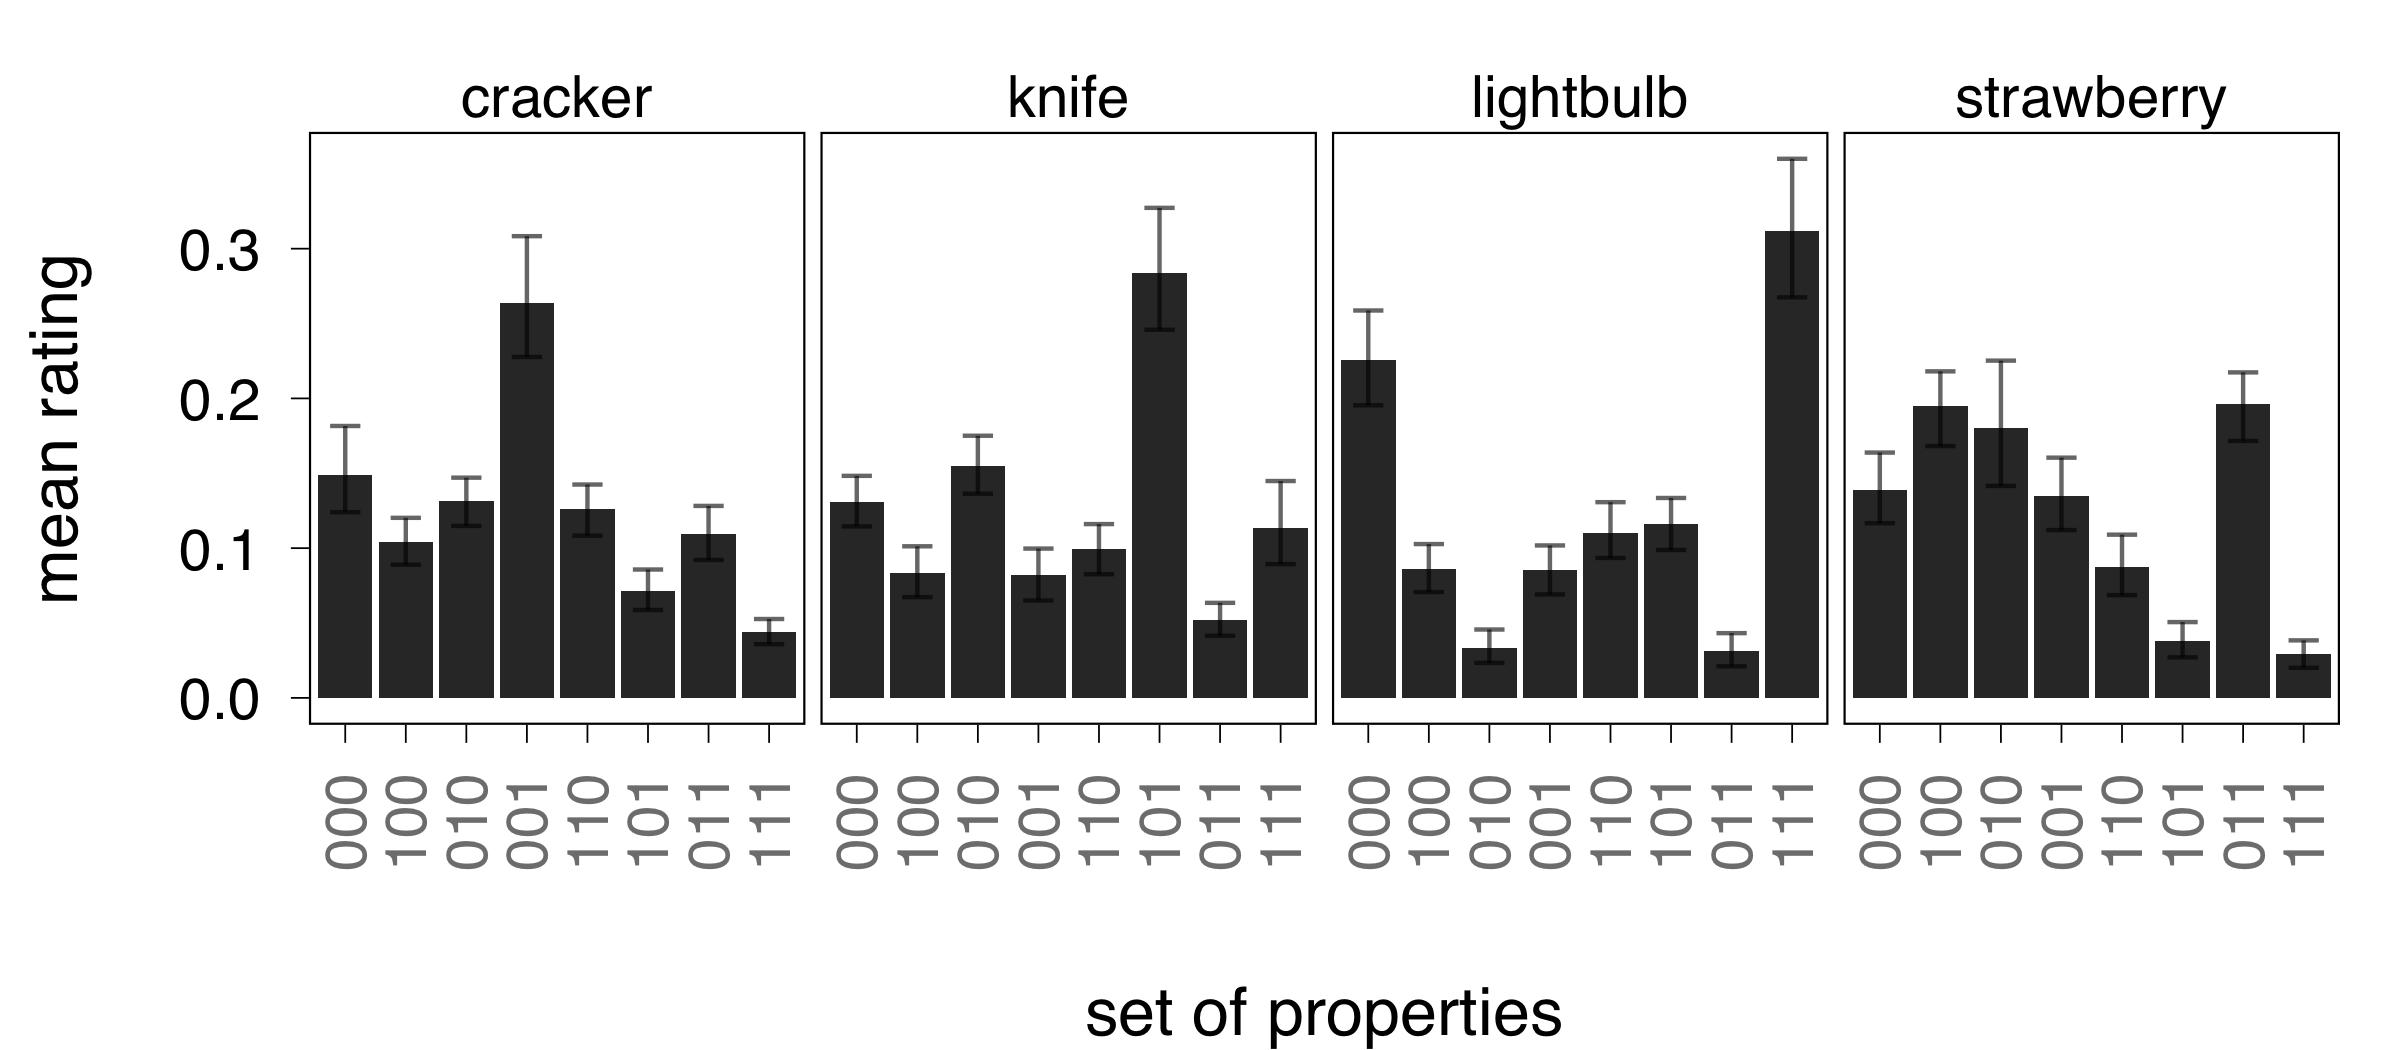
\includegraphics[width=\columnwidth]{priors}
    \caption{Mean elicited priors, collapsed across frequency and plausibility dependent measure (see main text). X-axis shows presence or absence of each property, the ordering of which can be found in Table \ref{tab:domains}.}
  \label{fig:priors}
\end{figure}



%$P(\delta_{\denote{c}(x)})$ is used because the model of argument strength isn't given a conclusion, but rather \emph{generates} a conclusion according to the prior distribution over situations. $P(\delta_{\denote{c}(x)})$ ensure that a conclusion wihich is true of the 


%For concreteness, assume that the number of objects in a situation is 4. The relevant number of objects that satisfy the a premise will depend on that particular premise. For example, \emph{All of the grey elephants are herbivores} is true if all of the elephants that are grey in the particular situation are also herbivores\footnote{N.B. I use the ``of the'' construction to make clear that I am describing a particular situation of elephants and not elephants in general.}. The model is given some number of elephants: in our example, 4. The model then samples properties \emph{grey, herbivore} according to the joint prior distribution of these properties $P(x) = P(g,h)$. Depending on the prior probabilities of $g$, a given situation may have 0, 1, 2, 3, or 4 grey elephants. The premise that \emph{All of the grey elephants are herbivores} is evaluated with respect to the number of grey elephants in that situation. If there are 3 grey elephants, then $\denote{\emph{All of the grey elephants are herbivores}]}: \forall{x}, g(x) \Rightarrow h(x)$

%and $S = \{s_0, s_1, s_2, \dots, s_{4}\}$, where the subscript indicates the number of objects (e.g., marbles) that exhibit an effect (e.g., sinking). 
%Further assume that the set of utterances \emph{All/None/Some of the marbles sank} is denoted $U = \{u_{\textrm{all}}, u_{\textrm{none}}, u_{\textrm{some}}\}$ and each has its usual literal meaning: 
%%$\denote{u_{\textrm{none}}}: s=0$,  
%%$\denote{u_{\textrm{some}}}: s>0$,
%%$\denote{u_{\textrm{all}}}: s=15$.
%$\denote{u_{\textrm{none}}}= \{s_i | i = 0\}$,  
%$\denote{u_{\textrm{some}}}= \{s_i | i > 0\}$,
%$\denote{u_{\textrm{all}}}= \{s_i | i = 15\}$.

\section{Experiment 2: Syllogistic reasoning about real world content}

In Experiment 2,  I sought to test if syllogisms using the real world content of Experiment 1 led to different conclusions.

\subsubsection{Design}

I recruited 254 participants from Amazon's Mechanical Turk. All participants were required to have a 95\% approval rating for their previous work on the web service. 

Each participant completed 4 syllogisms. Each syllogism was paired with a random domain used in Experiment 1.

A total of 8 syllogisms were used, resulting in 32 unique \{syllogism, domain\} pairs.

\subsubsection{Procedures \& Materials}

The instructions to the experiment were:

\begin{quotation}
In this experiment, you will read four (4) randomly selected logical arguments. For each argument, you will be presented with different conclusion that might follow from the argument presented.
\end{quotation}

On each experimental slide, the participants saw the words ``Given that:'' followed by the syllogism. Below was written: ``Does it follow that:''. Below that was presented a 4 column table with each of the 4 syllogistic conclusions in a column. Below each conclusion was the dependent measure. The dependent measure was a radio button with the options ``Doesn't follow'' and ``Follows''. Below that was a vertically-oriented slider bar with endpoints labeled ``Certain'' and ``Don't know''. 

\begin{quotation}
If you think the conclusion follows from the argument, indicate so. Adjust the position of the slider bar to reflect your confidence in your response.
\end{quotation}

Participants were required to mark each conclusion before continuing on to the next page.

\subsubsection{Results}

For a first pass with data analysis, I analyzed only the radio buttons. Shown in Figure \ref{fig:syllogismXdomain} (light bars) are the results of the experiments. There were effects of content and of syllogism on conclusions drawn, as evidenced by the differences in row and columns, respectively.

\section{Bayesian data analysis}

I compared the predictions of the TG model using the priors elicited in Experiment 1 to the reasoning data in Experiment 2. TG takes the probabilities to represent actual persons in a communicative setting, and so takes conclusions or premises to be selected from these distributions according to a Luce choice, or softmax, decision rule with a parameter that denotes the degree to which utterances are chosen optimally\cite{Luce1959}. This is one of the parameters of the model. The other parameter is the number of objects ($n$) parameter, which controls how large the worlds are that the reasoner reasons over. Results are highly consistent for $n \geq 4$ and I so use $n=4$ for all simulations.  

I put a uniform prior over the optimality parameter $\lambda \thicksim U(0,5)$. In addition, I use a data analytic ``guessing'' parameter $\phi \thicksim U(0,1)$ to account for response noise.

\subsection{Model comparison}

To address the relevance of background knowledge in syllogistic reasoning, I performed a Bayesian model comparison between models of argument strength with and without the empirical priors. The model without the empirical priors uses a Binomial prior with a parameter $br$ representing the base rate of properties\footnote{This is exactly the model of argument strength used in \citeA{Tessler2014}}). I put an uninformative Beta prior over the base rate parameter.

I put a uniform prior over the two models. Inference was done via the Metropolis-Hastings algorithm implemented in the probabilistic programming language WebPPL \cite{dippl}. The posterior probability of the model uses the empirical prior was . This suggests that it's highly likely that incorporating structured background knowledge into the model of syllogistic is necessary to capture human reasoning patterns.

To address the question of whether or not pragmatic (or, recursive) reasoning is still a necessary component of the model after accounting for background knowledge in the appropriate way, I compared the model of argument strength with the empirical prior with the model of pragmatic syllogistic reasoning with the empirical prior. 

I put a uniform prior over the two models. The posterior probability of the model that takes does pragmatic reasoning over an empirical prior was 0.984. This suggests that it's highly likely that this is a better model of the data than the model of argument strength. 

\subsection{Posterior predictives}

The model of pragmatic syllogistic reasoning was the most likely model in this space of models given this data. The posterior predictive distribution marginalizes over the inferred parameter values to produce predictions about what the data should look like given the posited cognitive model and the observed data. This is akin to fitting the parameters and is an important step in model validation as it shows what data is actually predicted by the model.

The overall correlation between the posterior predictive and the human data was $r = 0.85$ (Figure \ref{fig:scatterplot}). The Syllogistic RSA model captures many of the qualitative patterns in the reasoning data, as well (Figure \ref{fig:syllogismXdomain}). 

\begin{figure}
\centering
    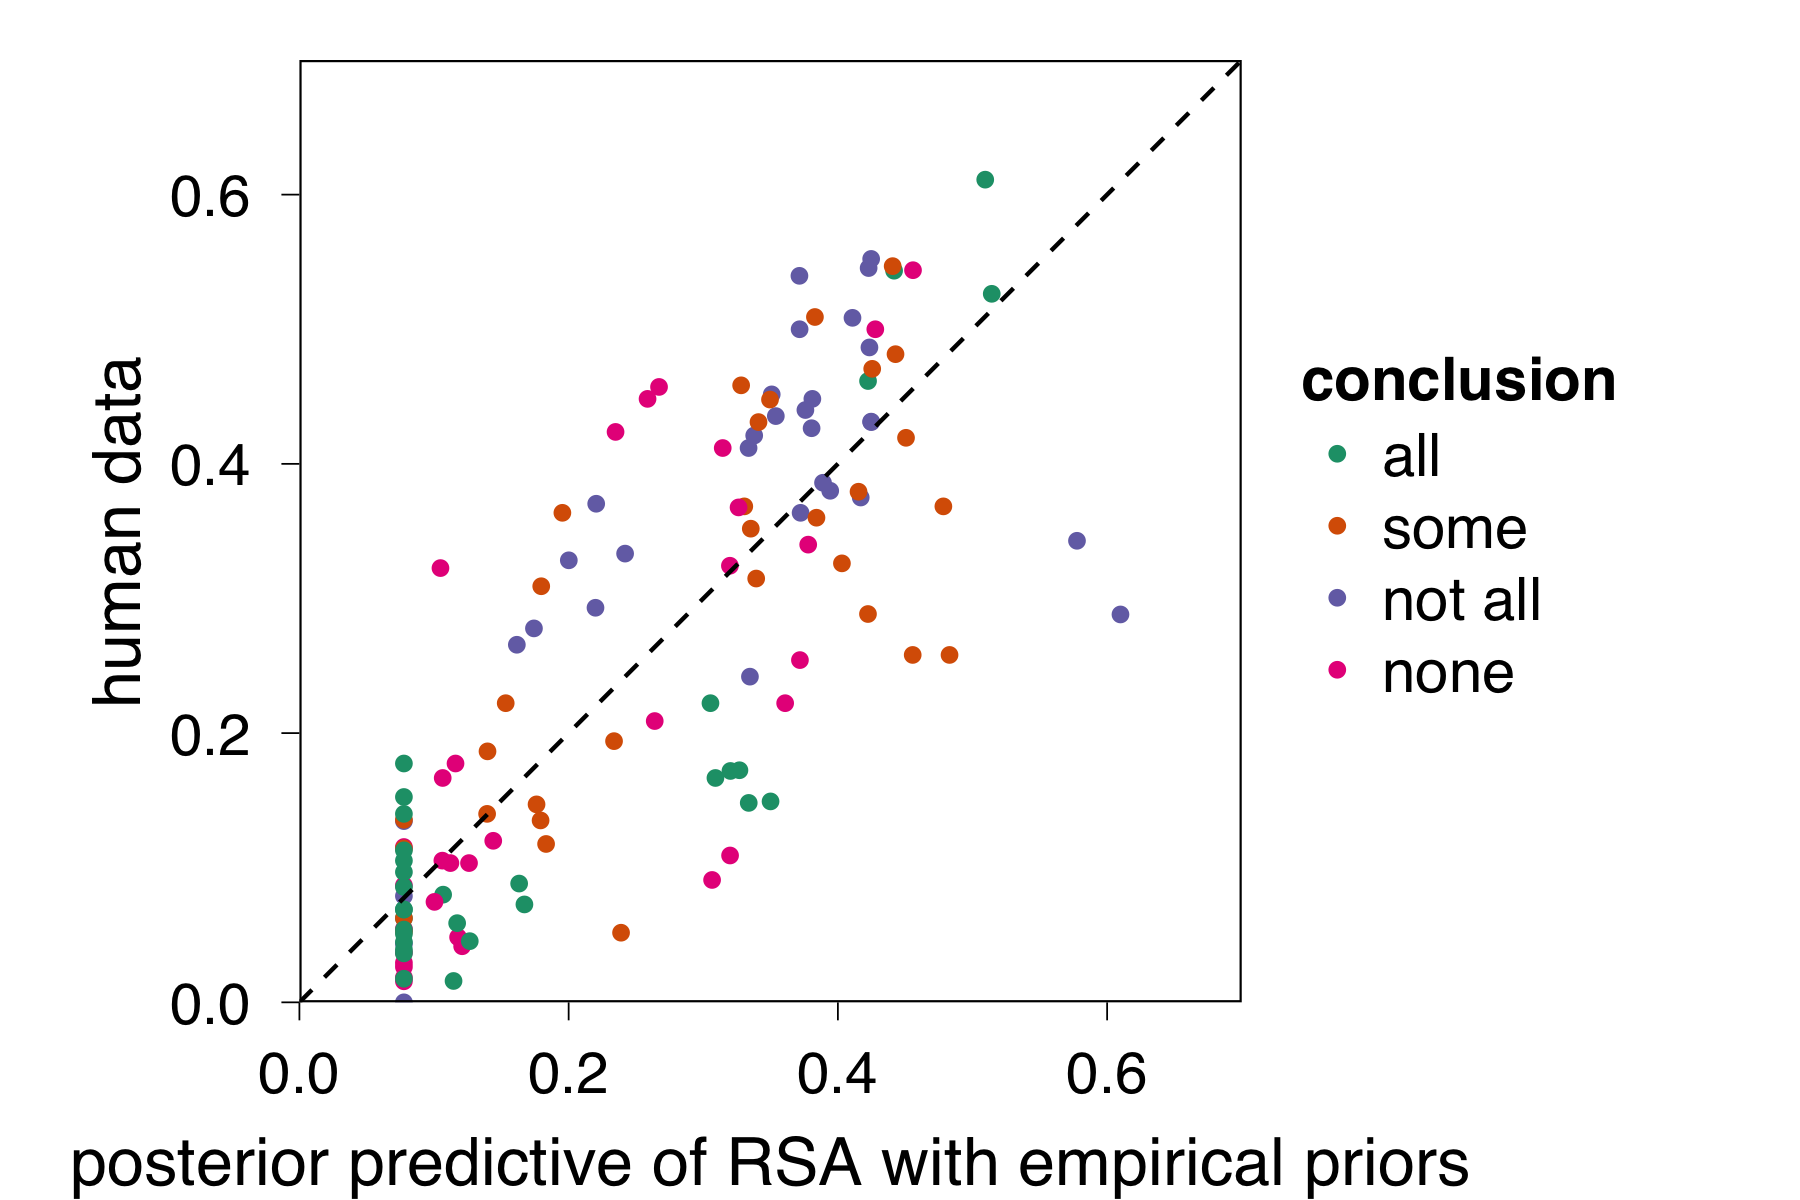
\includegraphics[width=0.5\columnwidth]{figures/scatterplot}
    \caption{Data vs. Model plot. The model provides a good overall fit to the 128 data points (32 syllogism, domain pairs X 4 conclusions each). The posterior predictions bottom out around 0.07. This is the work of the response noise parameter $\phi$. It's likely that different syllogisms have different amounts of response noise, however I do not model this here.}
  \label{fig:scatterplot}
\end{figure}

\begin{figure}
\centering
    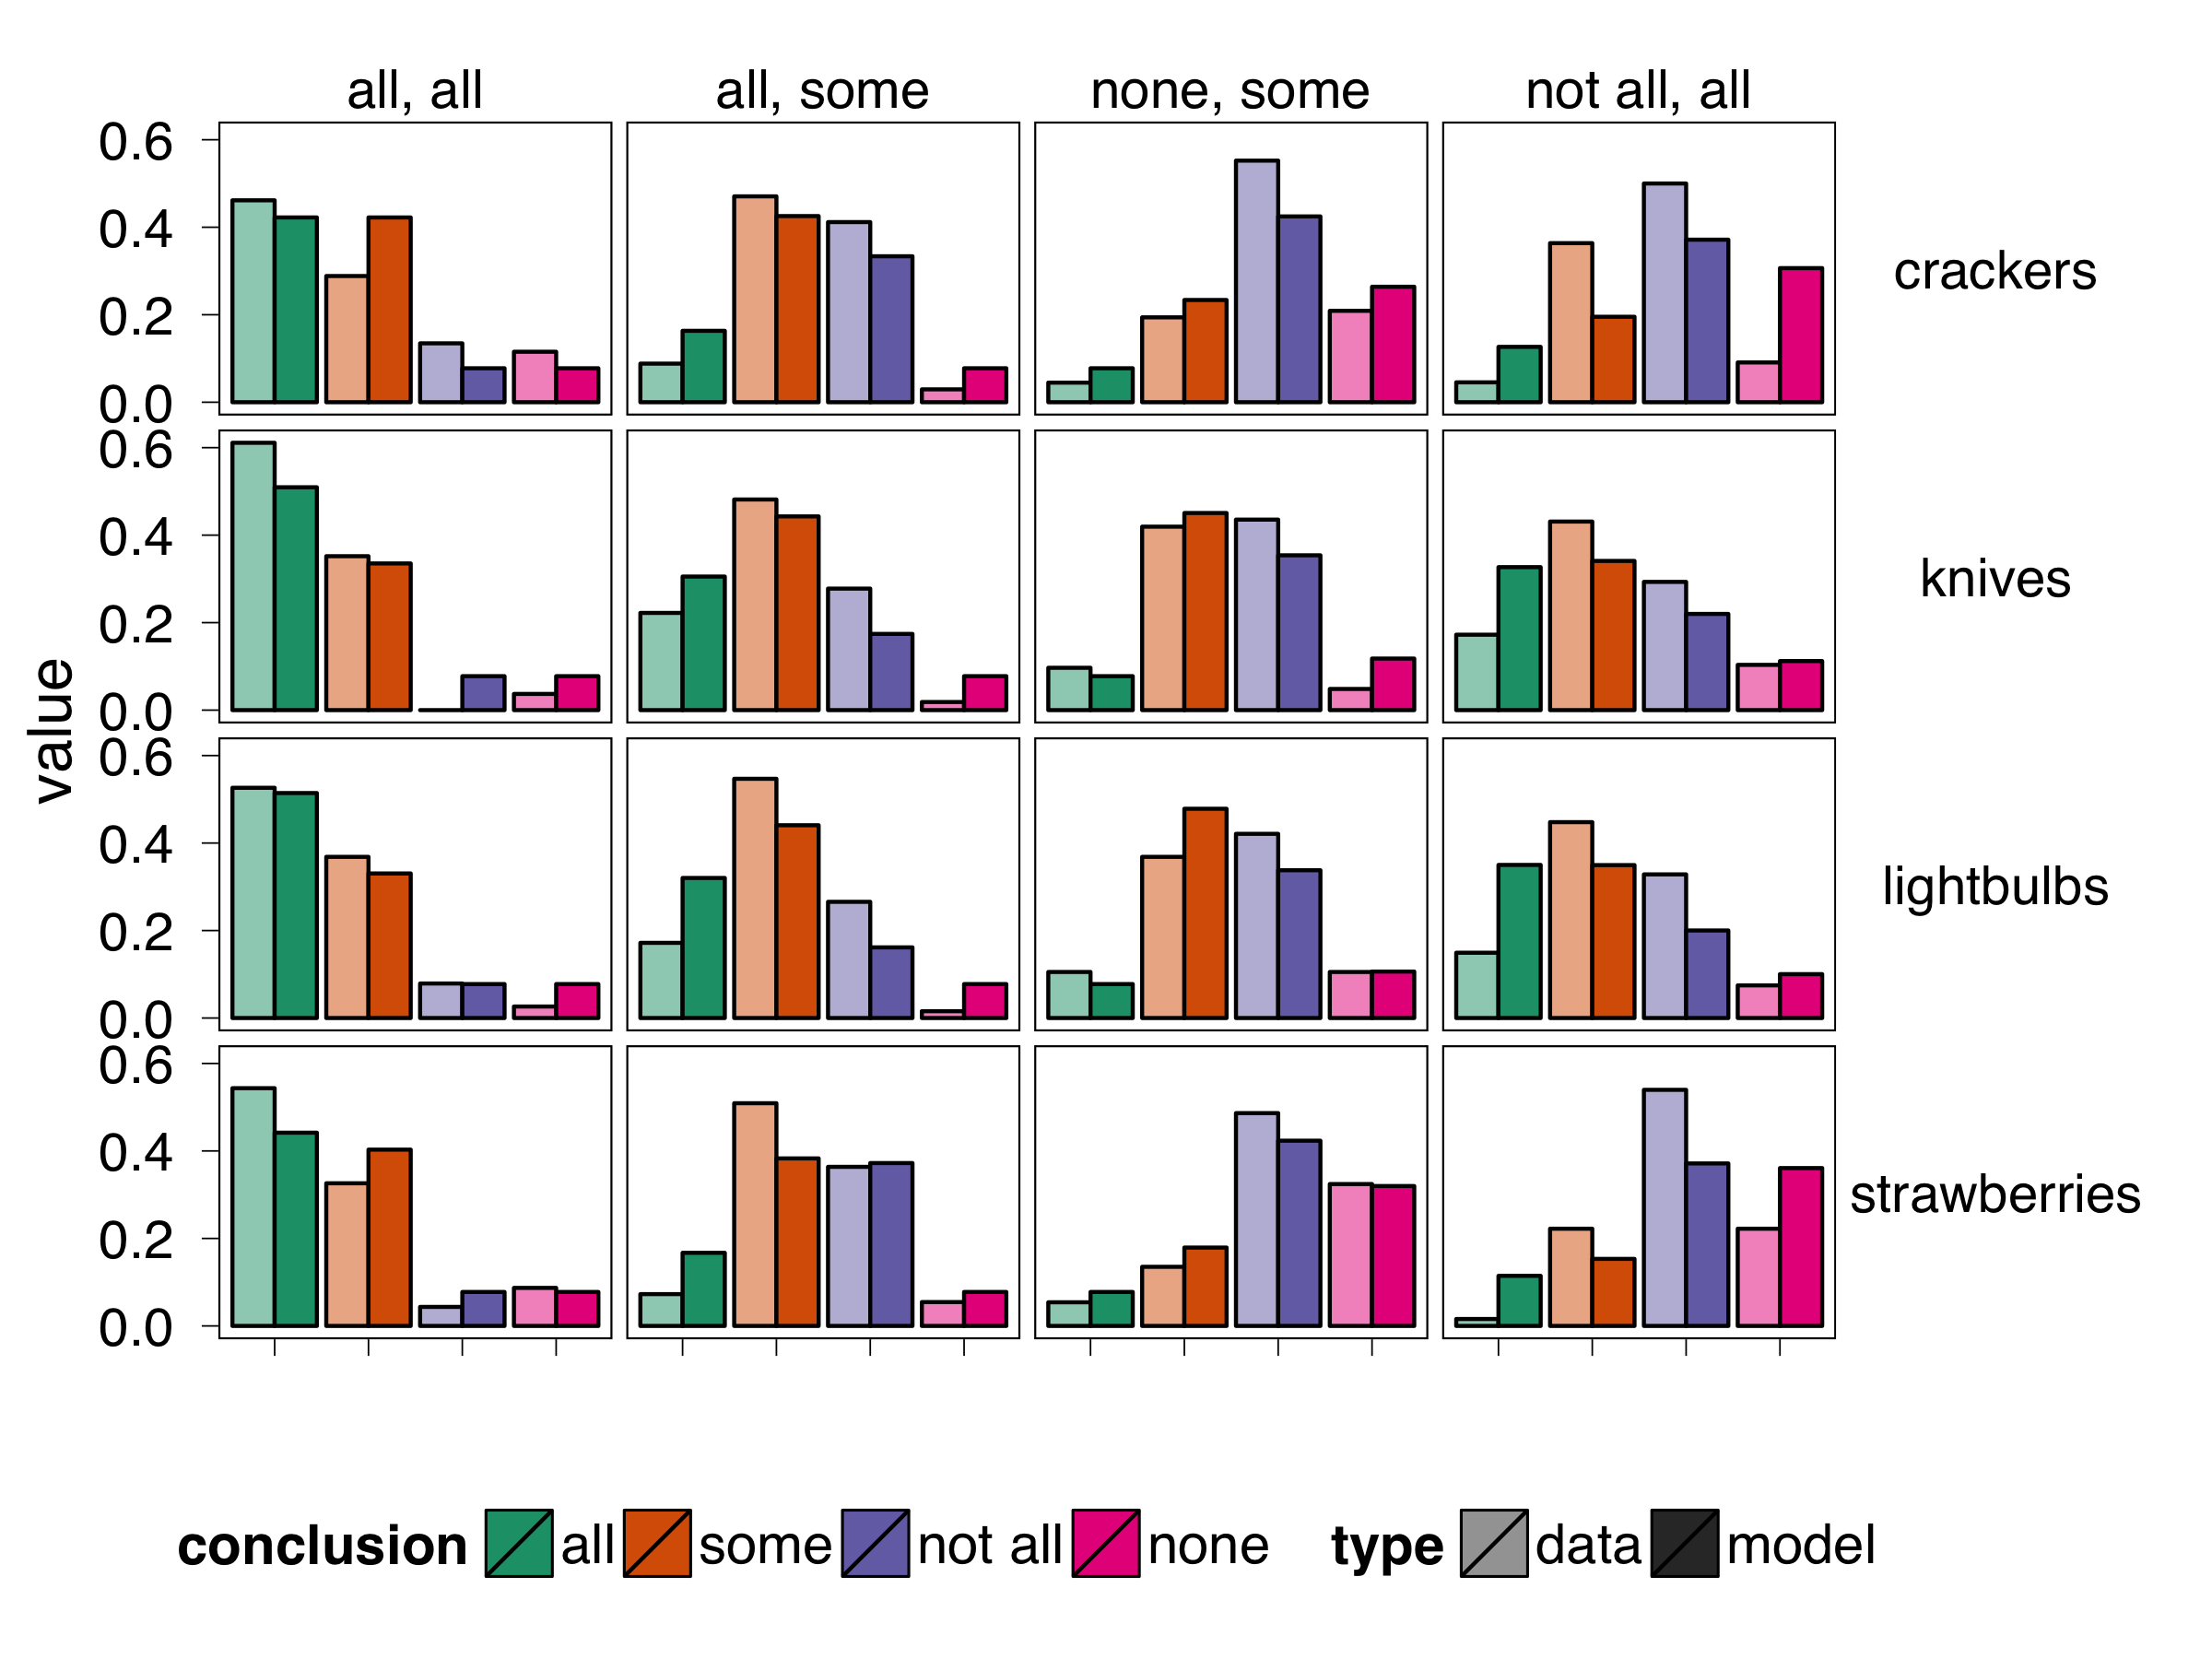
\includegraphics[width=\columnwidth]{figures/syllogismXdomain}
    \caption{Reasoning patterns and predictions for 4 (of the 8) syllogisms in Experiment 2. Model predictions are in the darker shade. All syllogisms shown here were of the form B-A / C-B and the conclusions were of the form C-A (e.g. second column: All B are A, Some C are B). Reasoning effects can be seen by comparing columns within a row. Content effects can be seen by comparing rows within a column.}
  \label{fig:syllogismXdomain}
\end{figure}

\section{Discussion}

I have demonstrated in this paper that a model of syllogistic reasoning requires the appropriate prior distribution to account for the flexibility of interpretation of a syllogistic argument with real world content. The prior distribution is not enough, however. The recursive nature of communicative inference needs to be taken into account to capture the deviations from a literal semantic interpretation of the premises. 

%\subsection{Wonky worlds?}
%\section{Conclusion}

\bibliographystyle{apacite}

\bibliography{belief}

\end{document}
